\section{Baseline Competitors}
To show the performance gain archived by our proposed solution in section \ref{sec:contribution} we use 2 baseline competitors.
The 2 competitors are chosen as they use simple and well known caching techniques. Both competitors take advantage of the optimal substructure property of the cached shortest path items.

\subsection{LRU}

LRU - Least Recently Used. This competitor uses the LRU cache replacement policy which gives each cache item a timestamp when it is added to the cache, and updates the timestamp if the cache item contributes to a cache hit. When a \spath query does not generate a cache hit, the new \spath will trigger a cache replacement. LRU simply throws out the cache item with the lowest timestamp and adds the new cache item with the current timestamp.

\subsection{FIFO}

FIFO - First In First Out. FIFO replaces, as the name suggests, the oldest cache item when a new \spath item is calculated and needs to be added to the cache. FIFO is the simplest of the suggested cache replacement policies.




\section{\spath algorithm speedup} \label{sec:contribution}

The techniques proposed here will each present how, and in what way, they can contribute to fulfilling sub-goal 1, set out in section \ref{subsec:goals}.

All cache replacement techniques presented takes advantage of the optimal substructure property of shortest path, so all items in the \spath cache can also answer queries which only need a part of the shortest path.

% % The current section "5.1.1 Cache Replacement Policies"
% %    should be divided into two subsections:
% % 
% % - 5.1.1 Optimal Substructure Cache
% %   ( Here, you talk about the caching example on page 4)
% % 
% % - 5.1.2 Cache Replacement Policy
% %   ( Here, you talk about the "scoring mechanism".  You can then add an example to illustrate how this policy works. )
\subsection{Cache Replacement Policies}

By using a cache a replacement policy, we try to directly shorten the total execution time by reducing the number of times the \spath algorithm has to be executed. 
The execution time is shortened every time we have a cache hit since the \spath algorithm\footnote{This can be any \spath algorithm, and we a just referring to the general set of \spath algorithms} does not need to run, and \spath algorithms usually are quite expensive in terms of the number of calculations and/or comparisons it needs to do to produce a result.


\subsubsection{\osc}

The basis of \osc is two scoring mechanisms which can either be added or multiplied to each other to assign each cache item a score. \osc does cache replacement based on the calculated score. If a new cache item get a lower score than any of the existing cache items it will not replace any existing cache items and will be discarded, if one or more items exist in the cache which have a lower score than some new candidate, then the item with the lowest score will be replaced (Fig. \ref{fig:advancedroutequery}, step D).

\begin{lemma}{\it \textbf{\spath Optimal Substructure}}
Given a weighted DAG $G = (V, E)$ let $p = \left< v_1, v_2,..., v_k \right>$ be a shortest path from vertex $v_1$ to vertex $v_k$ and, $\forall i,j | 1 \leq i \leq j \leq k$, let $p_{ij} = \left<v_i, v_{i+1},..., v_j \right>$ be the subpath of p from vertex $v_i$ to vertex $v_j$. Then, $p_{ij}$ is a shortest path from $v_i$ to $v_j$.
\end{lemma}



\subsection{Cache structures}

We will consider 3 basic cache structures, each with optional ways of using or implementing them. The 3 cache structures are briefly:
\begin{itemize}
\item A single array. A cache lookup means scanning the array.
\item A map on an array, quickly identifying valid candidates for a cache hit.
\item Using one of the two ideas already mentioned, but changing the structure of the cache items (\spath results) to use \spsns, sharing sub-parts, to conserve space.
\end{itemize}

\subsubsection{Array, Direct Access}

The simplest way to implement a cache is to just store all cache items in an array. An example of how the cache works is presented in  figure \ref{fig:cachestruc}, part A,D, and E. In figure \ref{fig:cachestruc}A two \spath queries, Q1 \& Q2, are submitted. By scanning the array in \ref{fig:cachestruc}D item 3 and 4 are identified as being able to answer Q1 and Q2. Cache item 3 contains a superset of the set of nodes needed to answer Q2 so in \ref{fig:cachestruc}E the answers are refined and sent back to the user.

While this cache structure is very simple and there for incurs virtually no overhead in terms of maintaining the structure, then the array needs to be scanned each time a new query is submitted to the system, and the entire array will be scanned if the query can not be answered by the cache. This cache structure has a high overhead because it needs to scan the array, and if the cache is large it is not likely to be an efficient solution or fulfill subgoal 2 very well (see Sec. \ref{sec:architec}).


\subsubsection{Array with Map, Indirect Access}
By adding a map with an inverted list on top of the array, holding the cache items, we can answer queries in constant time. The inverted list maps node ids to the cache items in which they are present. Figure \ref{fig:cachestruc}A-E shows how this works. In \ref{fig:cachestruc}A two queries are submitted. For each query we make a lookup in the map (fig.\ref{fig:cachestruc}B) for the start and end node of the query. In \ref{fig:cachestruc}C We then take the intersection of the possible cache items containing a shortest path with the start and end nodes of each query. If the were to be empty we would immediately know the cache can not answer the query. In \ref{fig:cachestruc}D we directly access the cache items identified in \ref{fig:cachestruc}C and refine them in \ref{fig:cachestruc}E before sending the answer back to the user.

This cache structure require some additional work to maintain, as the map needs to be updated each time the cache content changes i.e. when cache items are replaced, but otherwise incur very little overhead. This structure is expected to perform quite well and be very good at helping to fulfill subgoal 2 (see Sec. \ref{sec:architec}).

\subsubsection{Array with Shared Sub-paths}
To support the \sps idea presented before, new node type has been introduced (fig. \ref{fig:nodetypes}). Previously the cache items only consisted of a list of node ids. To support the idea of \sps two new node types has been introduced, node 0 and 1. Node type 0 is only a node id with a type 0. Node type 1 consist of a cache item id and the id of the start and end node which is shared between the two cache cache items.

\sps can be implemented on top of either of the two previously presented cache structures, as it only changes the internal way of storing the cache items. This idea incurs a substantial overhead each time a cache item has to be replaced, as it is needed to check whether the replaced cache item is sharing or being shared with other cache items. This method does however also free up more space, allowing for more cache items and hopefully fewer cache replacements.


\begin{figure}
  \center
	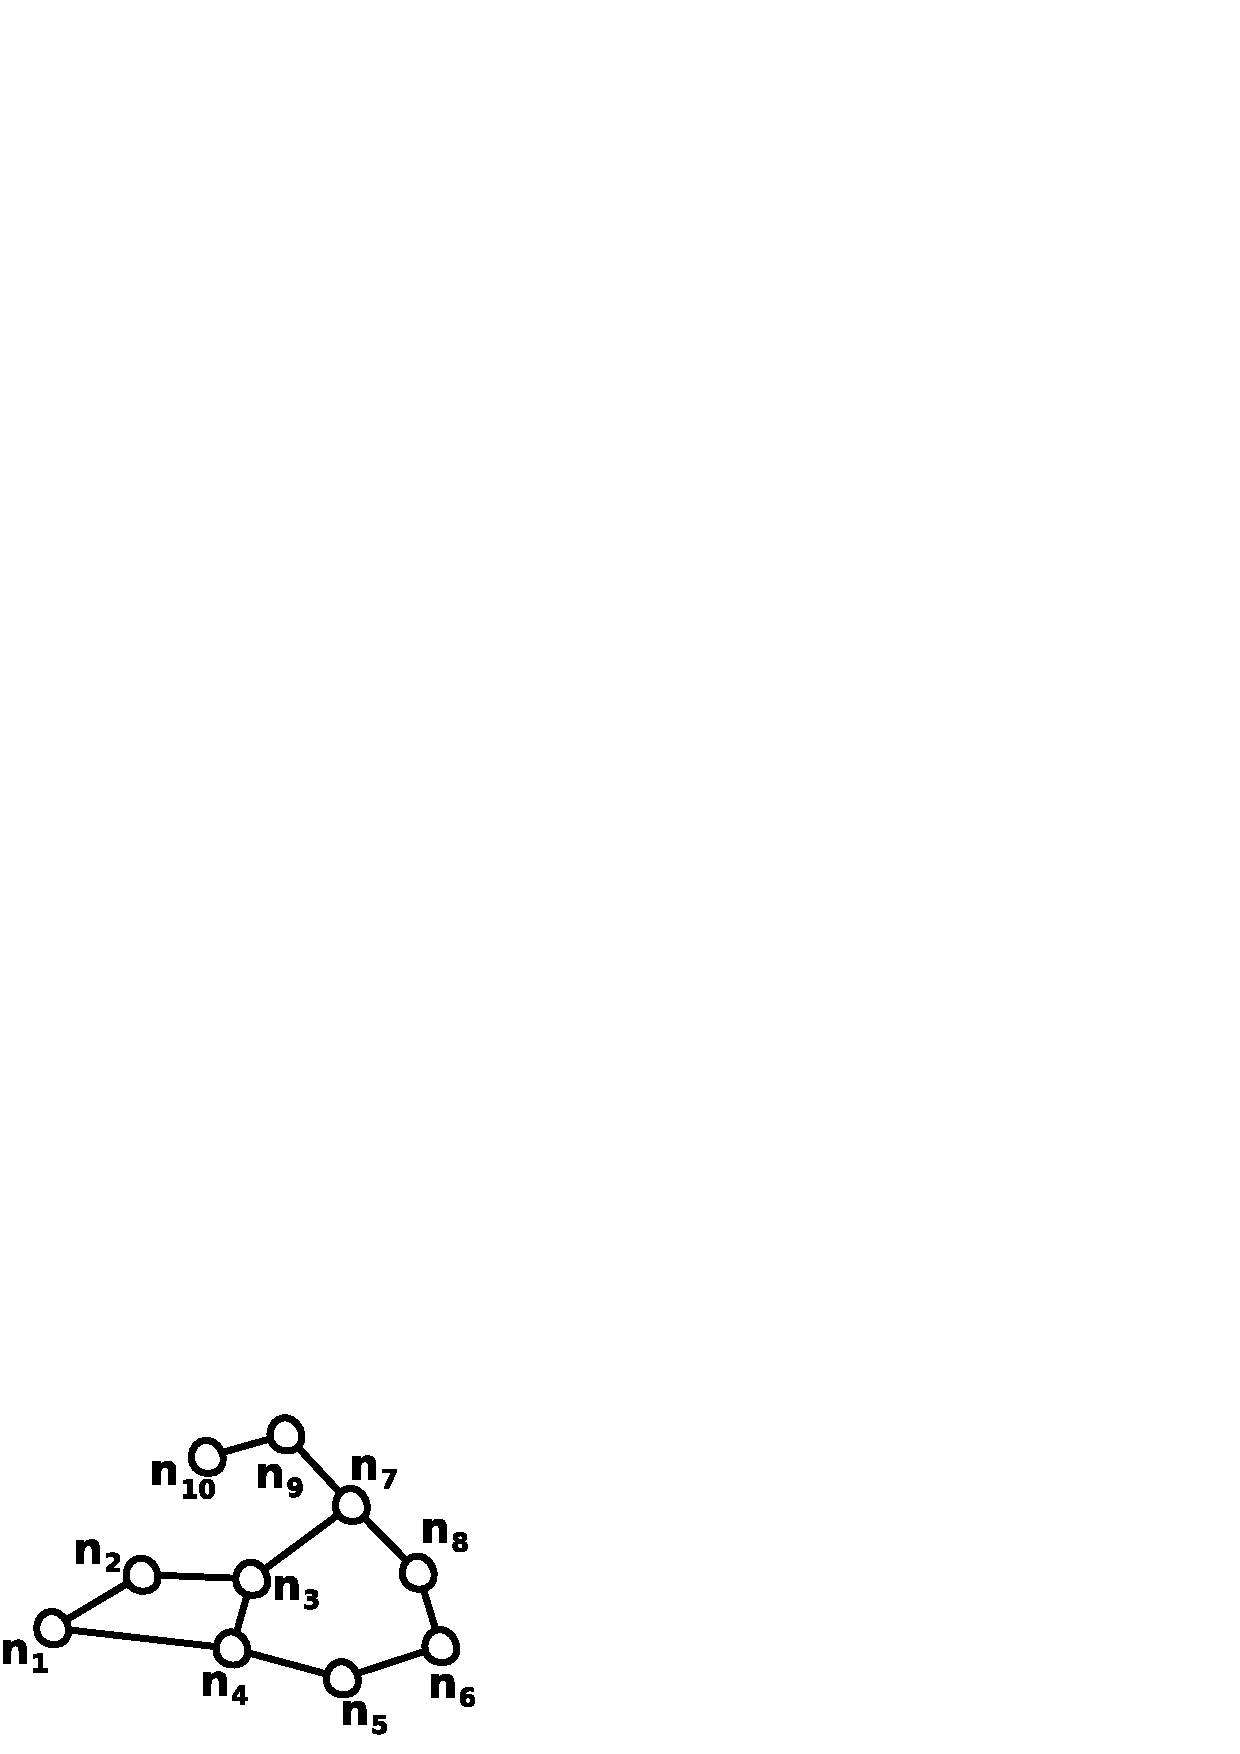
\includegraphics[width=0.3\textwidth]{figures/map10n.pdf}
	\caption{Map}
  \label{fig:map10}
\end{figure}

\begin{figure}
  \center
	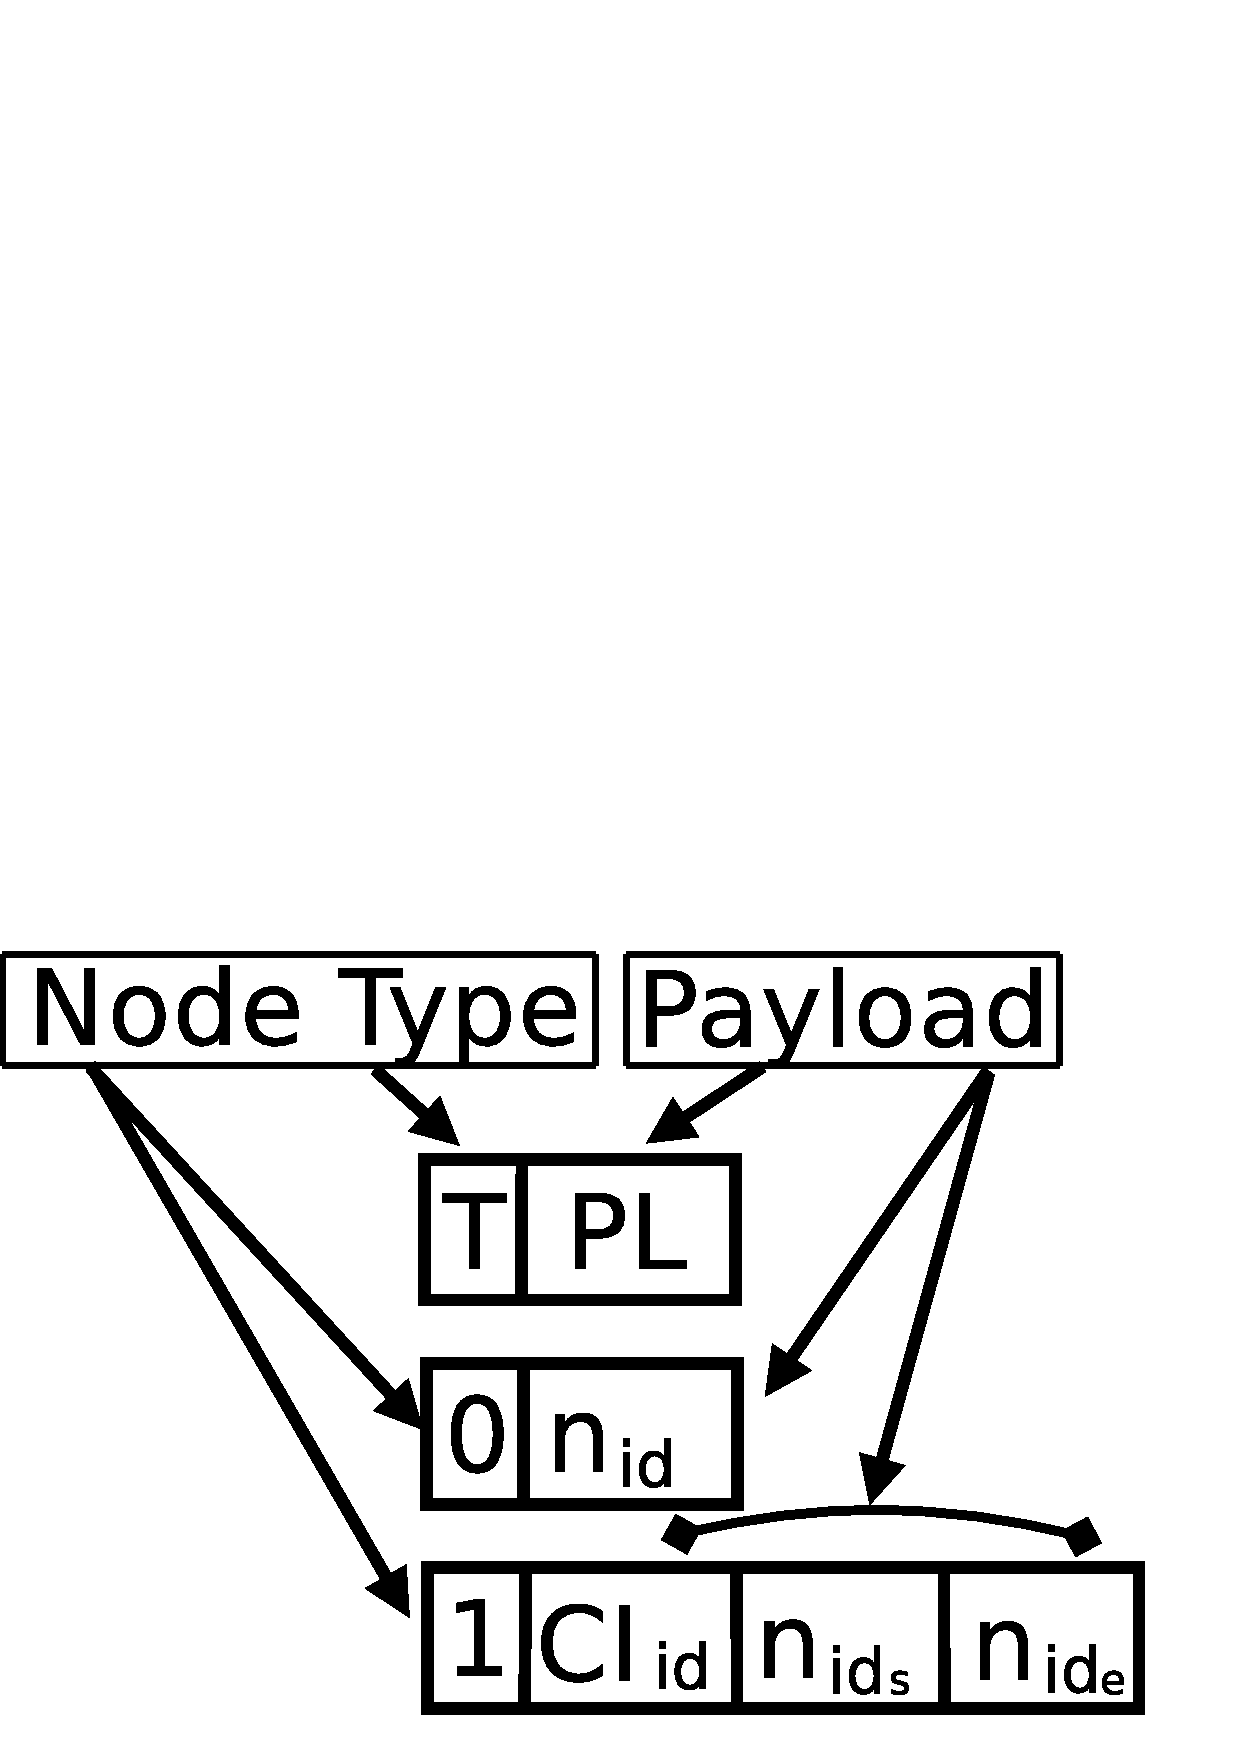
\includegraphics[width=0.3\textwidth]{figures/nodeType.pdf}
	\caption{Node types}
  \label{fig:nodetypes}
\end{figure}

\begin{figure}
  \center
	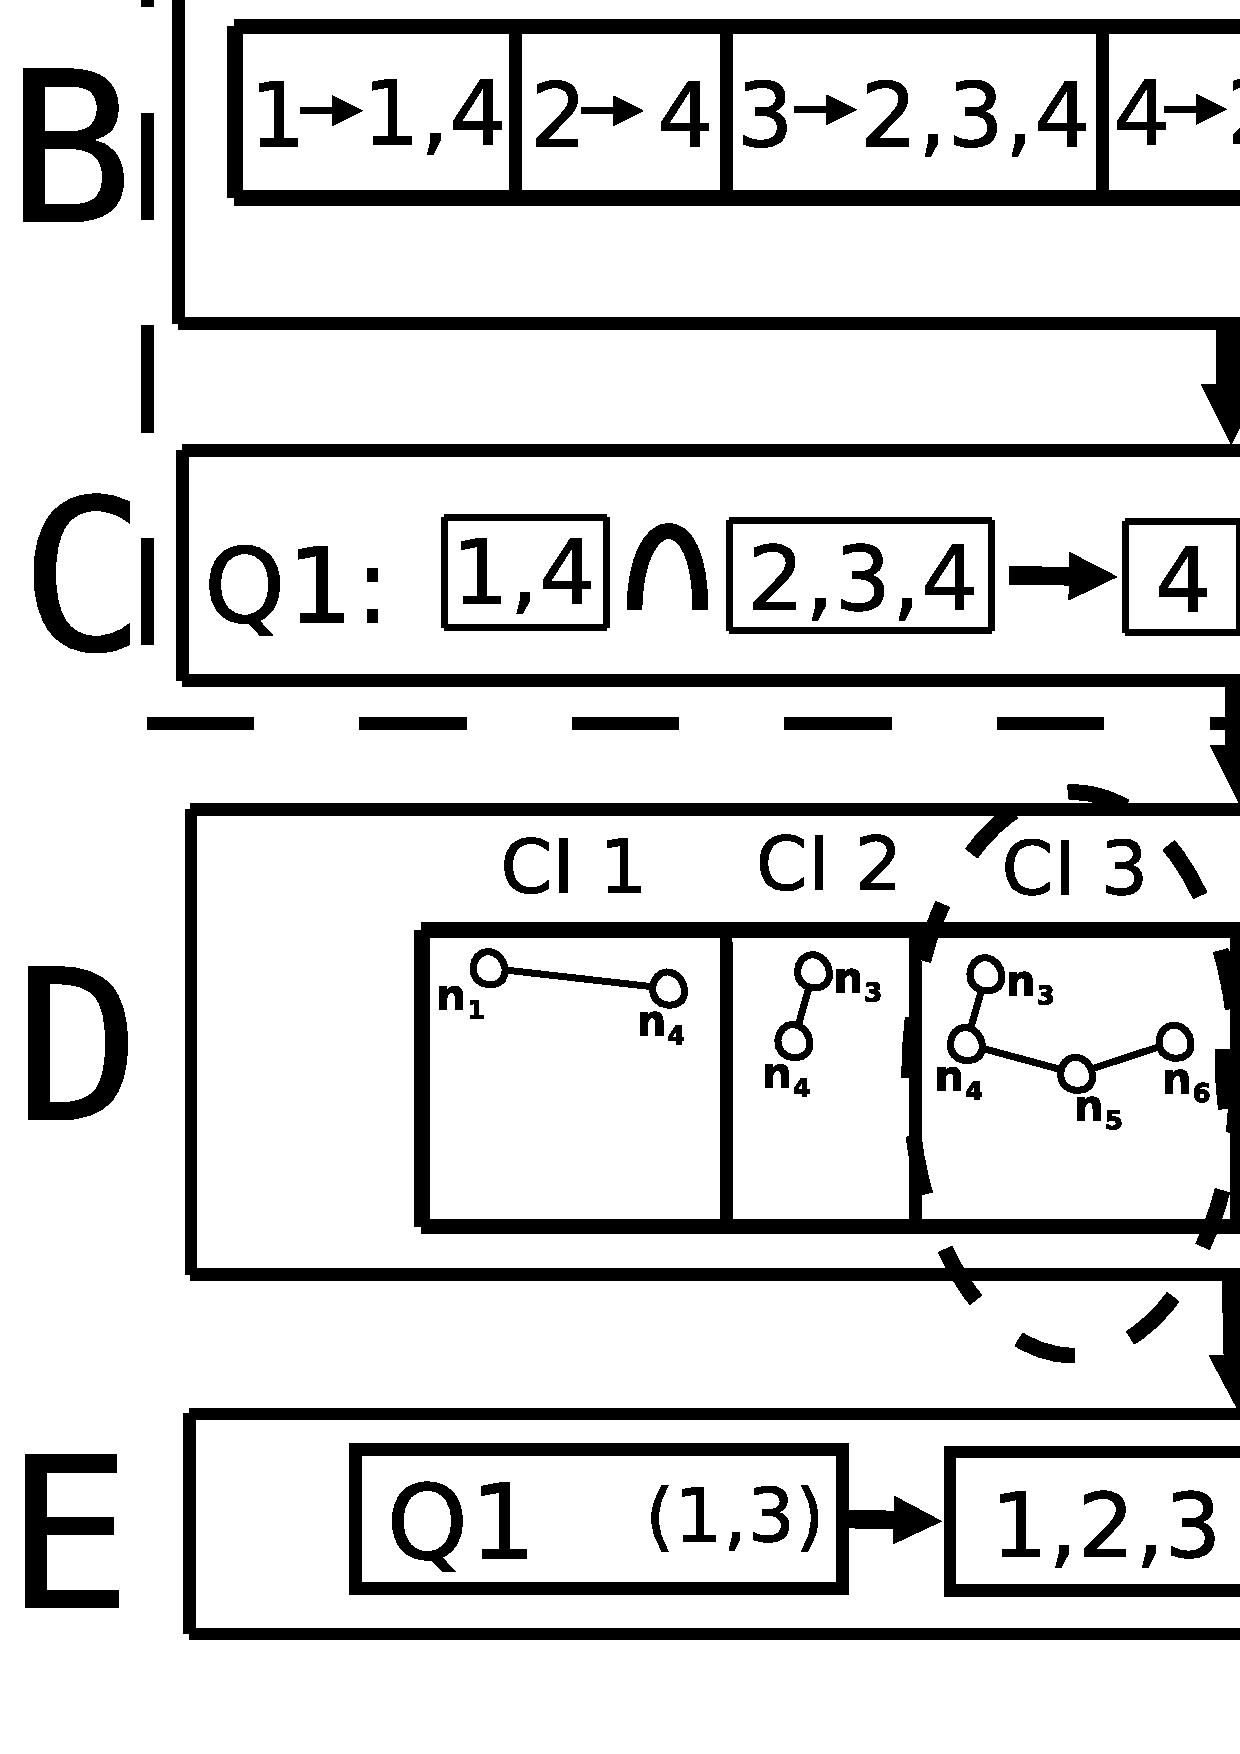
\includegraphics[width=0.52\textwidth]{figures/cacheTwoLayer.pdf}
	\caption{Cache access}
  \label{fig:cachestruc}
\end{figure}


\section{Overhead reduction}
The techniques proposed here will each present how, and in what way, they can contribute to fulfilling sub-goal 2, set out in section \ref{subsec:goals}.

\subsubsection{Scoring Mechanism}


The scoring is done by summing up: the number of times a cache item has formed the basis of a cache hit; the number of times each node in cache item has been the source/target nodes in a query, or member of a query result. By taking the length of a cache item (number of nodes in the \spath) and multiplying it on the previously calculated sum we get the full score.

In \osc we use a scoring mechanism to rank the usefulness of cached items. Table \ref{tab:score} shows 3 queries ($i$) seen at different frequency and with different length. $C(l)$ calculates the number of vertices visited when finding a shortest path with a \spath algorithm. Based on these numbers it is then possible to calculate the benefit of adding one of these \spath queries to the cache. To calculate the savings gained from caching one of the 3 queries, first the cost of a cache hit $c_{hit}$ is multiplied with the item frequency, $i_{freq}$. This is then added to the value of $C(l)$ and subtracted from the cost of the queries without a cache, $nocache$. E.g. Item 1 has higher frequency (item freq/$i_{freq}$) than item 2, but the saving of putting item 2 in cache is much higher:

The cost (nocache) of item one is: $11*100=1100$ and item two cost: $10*200=2000$. Assuming a cache hit cost $1$, then adding item one to the cache would save = $1100-(100+10*1)=990$, and item two would save $2000-(200+9*1)=1791$. 

\begin{equation}\label{eq:cachesaving}
saving = nocache - (C(l) + (i_{freq} * c_{hit}))
\end{equation}


\begin{table}
\begin{center}
\begin{tabular}{l|r|r|r}
\hline \bf i & \bf Item freq & \bf Item length & \bf C(l) \\\hline
1 & 11 & 10 & 100 \\
2 & 10 & 15 & 200 \\
3 & 2 & 15 & 2000 \\\hline
\end{tabular}
\end{center}
\caption{\spath queries ($i$), their frequency, length, and cost of calculating result($C(l)$)}
\label{tab:score}
\end{table}


\subsection{\sps}

If space consumption is a very high priority then \sps is one option to alleviate the problem. \sps changes the cache structure from $n_1, ... , n_n$ to $CI_{k\left[s-node\right]},CI_{k\left[e-node\right]}, n_{e-node+1}, ... , n_n$.\footnote{This example only shows how to share something in the front of an item, though adding them after or in the middle does not matter.}
I.e. including the start-/end-node of a range from another cache item. The advantage of doing this is a, possibly large, reduction in the space requirements for the cache. Maintaining such a cache would be quite expensive in terms of computation when changes occur, though the space saving would allow for more cache items which again would reduce the total running time. We will later show whether this overhead can really be offset by the additional number of cache items which would fit into the cache.


% how does it work?
% what goal does it fulfill?
% how does it fulfill the goal?
\subsection{Partitioning Map}\label{sec:partionmap}

Partitioning of map into large region to quickly be able to discard items in the cache, leading to less work when trying to find a cache hit. By discarding possible \spath cache candidates early we may save some time and computations.

\ffh{improve fig. \ref{fig:mappartition}}

\begin{figure}
  \center
	\includegraphics[width=0.30\textwidth]{figures/mapPartition.pdf}
	\caption{Partitioned Map}
  \label{fig:mappartition}
\end{figure}

\subsection{Partitioning Caching} 

The idea behind Partitioning caching builds upon the idea of partitioning the map (Sec. \ref{sec:partionmap}), but takes one step further. If a map can be partitioned in such a way that there is only one connection between them, then the connection can be cached and there by greatly reduce the search space needed to calculate a route between the two map partitions. The idea is shown in fig \ref{fig:cacheB}, \ref{fig:cacheA} where the search space needed to calculate a route from A to B is greatly reduced in fig. \ref{fig:cacheA} by caching partition 2.
\ffh{remember to equation to show by how much}

\begin{figure}
  \center
	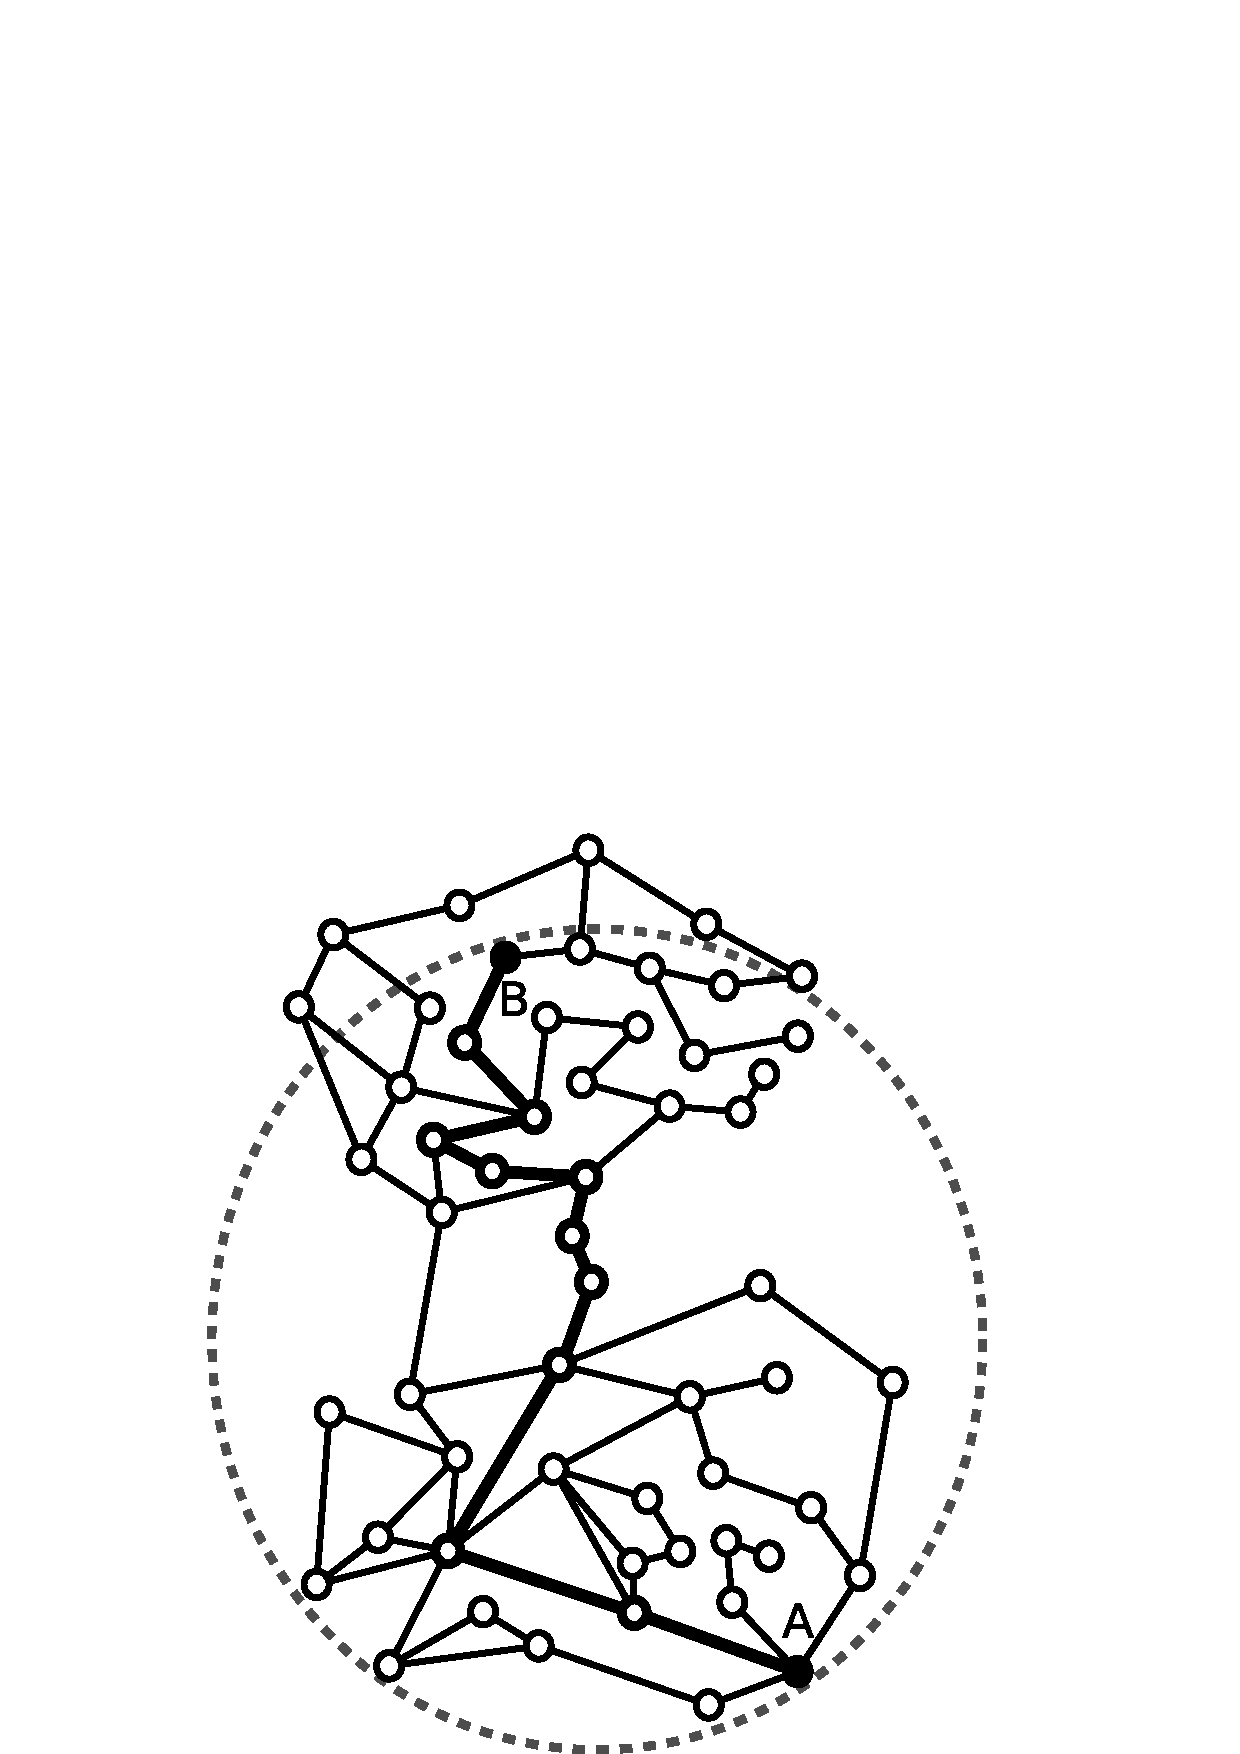
\includegraphics[width=0.42\textwidth]{figures/partSPcacheB.pdf}
	\caption{Normal SP searching area}
  \label{fig:cacheB}
\end{figure}

\begin{figure}
  \center
	\includegraphics[width=0.42\textwidth]{figures/partSPcacheA.pdf}
	\caption{Reduced SP search area (1 \& 3) based on partition caching (2)}
  \label{fig:cacheA}
\end{figure}


% % % % % % % % \subsection{Text and ideas which may still be useful (not part of paper)}
% % % % % % % % 
% % % % % % % % \ffh{need to focus on arguing about archiving lowest possible run time, do not connect to strongly with one map/graph, argue independently of map/graph that cost model and methods will be good.}
% % % % % % % % 
% % % % % % % % 
% % % % % % % % 
% % % % % % % % Figure \ref{fig:simplemap} shows a simple graph which we will use as our map and figure \ref{fig:simpleroutequery} shows the simple scenario in which a user (fig. \ref{fig:simpleroutequery}A) issues a route-planning query from 1 to 4 (fig. \ref{fig:simpleroutequery})  to an online route-planning server with a build in cache (fig. \ref{fig:simpleroutequery}B).
% % % % % % % % 
% % % % % % % % \subsubsection{Baseline}\label{baselinemethod}
% % % % % % % % \ffh{no longer used, but might be okay to use some parts for some motivation of why we want to do caching, or an intro to how the system works.}
% % % % % % % % The strait forward baseline solution is illustrated in figure \ref{fig:simpleroutequery}B. The idea is a server side shortest path cache which will store each query result in the cache and only consider exact query matches as cache hits, and to only use a simple cache policy such as LRU or FIFO.
% % % % % % % % The advantage of this solution is clear: it is simple and easily implemented. 
% % % % % % % % This simplicity is however obviously also it's main disadvantage, as it is too simple and very inefficient in terms of the utility the cache provides. Using items in the cache only when there is an exact match makes it exceedingly unlikely to get a cache hit due to the nature of route planning (many people share parts of routes, but few the same start and end points) and the sheer number of start-/end-point combinations possible.
% % % % % % % % 
% % % % % % % % \begin{figure}
% % % % % % % %   \center
% % % % % % % % 	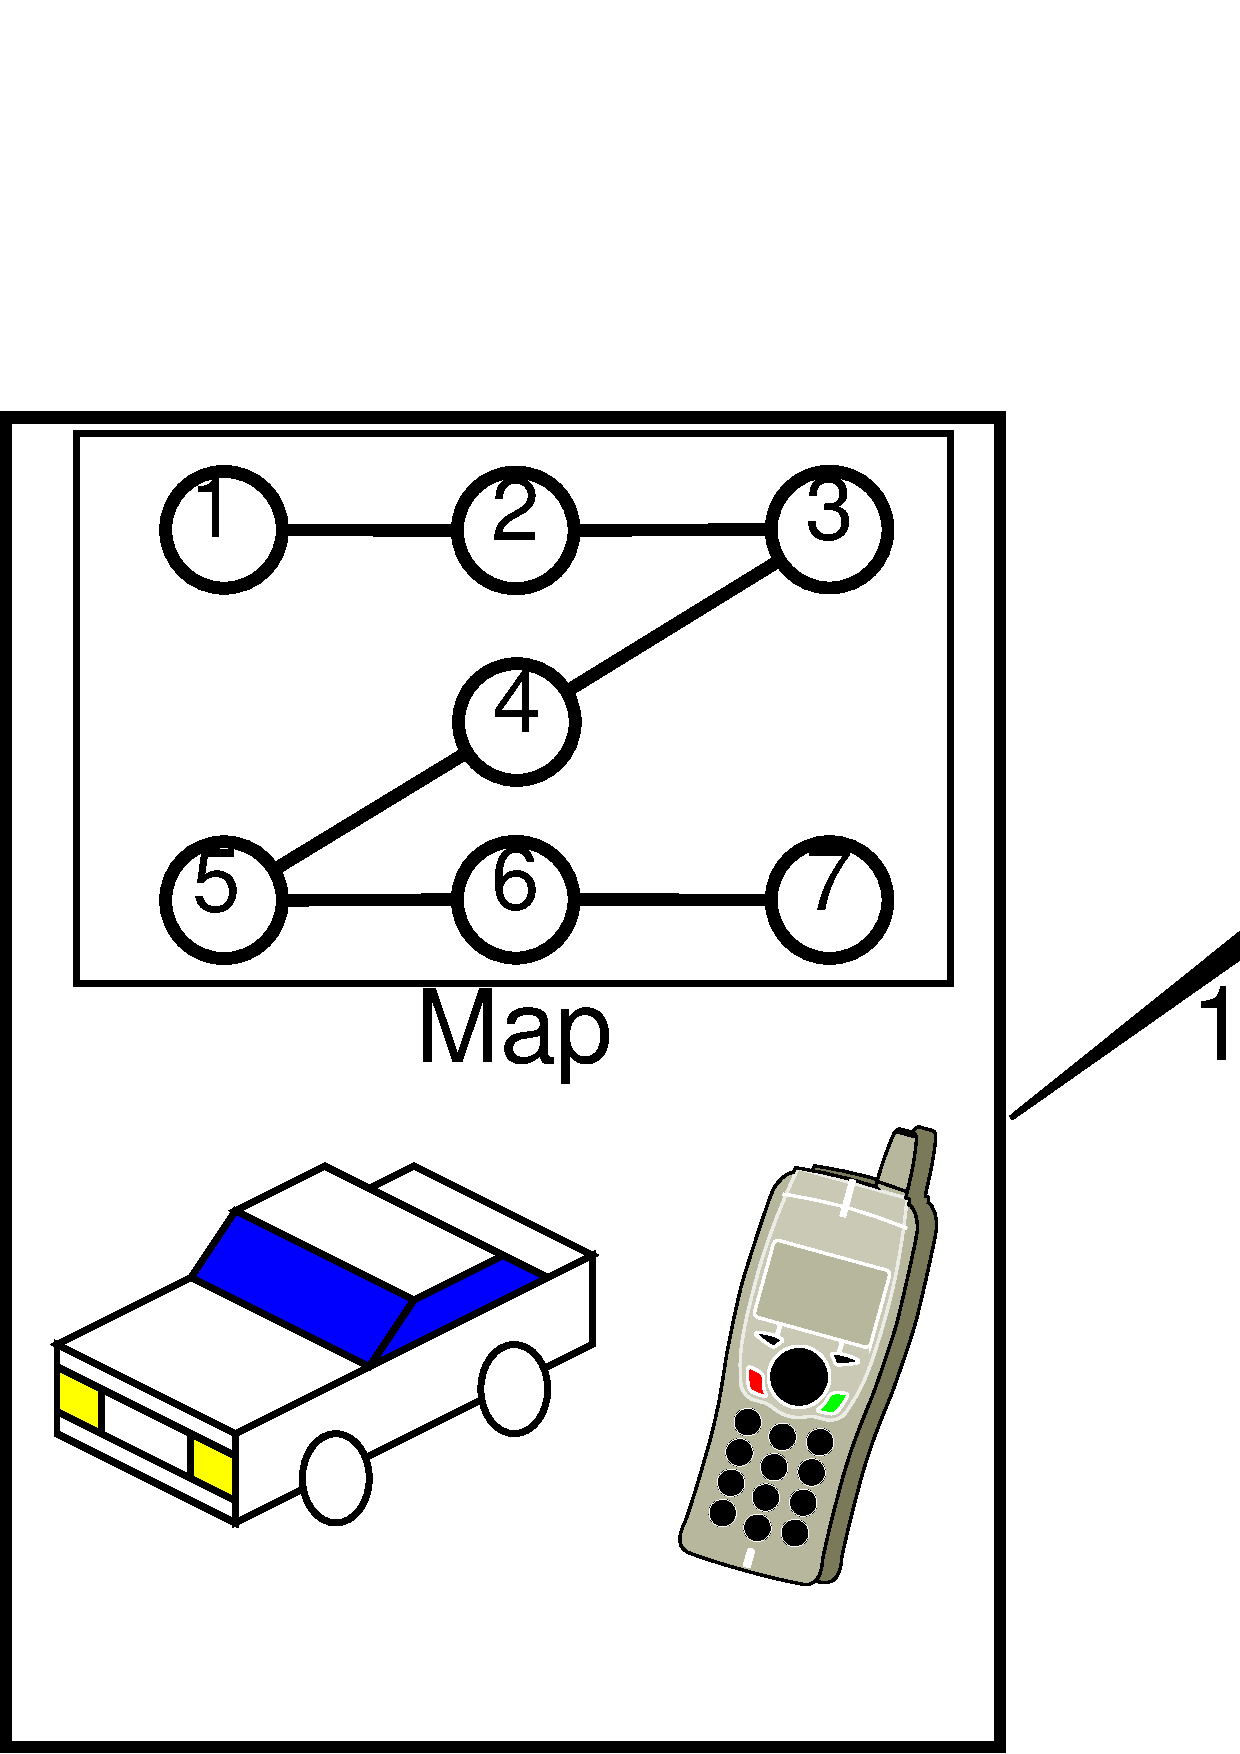
\includegraphics[width=0.5\textwidth]{figures/simpleroutequery.pdf}
% % % % % % % % 	\caption{simple graph}
% % % % % % % %   \label{fig:simpleroutequery}
% % % % % % % % \end{figure}
% % % % % % % % 
% % % % % % % % \subsubsection{Improved Baseline}\label{baselinemethodimp}
% % % % % % % % \ffh{no longer used, but might be okay to use some parts for some motivation of why we want to do caching, or an intro to how the system works.}
% % % % % % % % One way to possible increase the utility of a naive cache as proposed in \ref{baselinemethod} would be to exploit the \textit{optimal substructure property}\cite{introalg} of the cache items.
% % % % % % % % There is a significant increase in cache hits to be expected by utilizing the optimal substructure of shortest path cache items since it is unlikely many people will plan a route from/to the same place, but it is very likely that some sub-parts will be shared among users, and some users' full path laying within a longer path already calculated. The idea is illustrated in figure \ref{fig:cacheQueries} where the baseline method would be able to answer query Q1 from the cache, but not Q2. It is this specific disadvantage which ImpBaseline addresses and ImpBaseline can therefor answer both Q1 and Q2 from the cache since the result of Q2 now exist as a solution to a subpath of cache item C3.
% % % % % % % % Doing this adds a need for additional computational resources \ffh{how many resources?} required to examine the substructure of each  cached shortest path search result. It is currently not known if doing this is worth the effort, compared to just calculating the route, possibly multiple times.
% % % % % % % % 
% % % % % % % % \begin{figure}
% % % % % % % %   \center
% % % % % % % % 	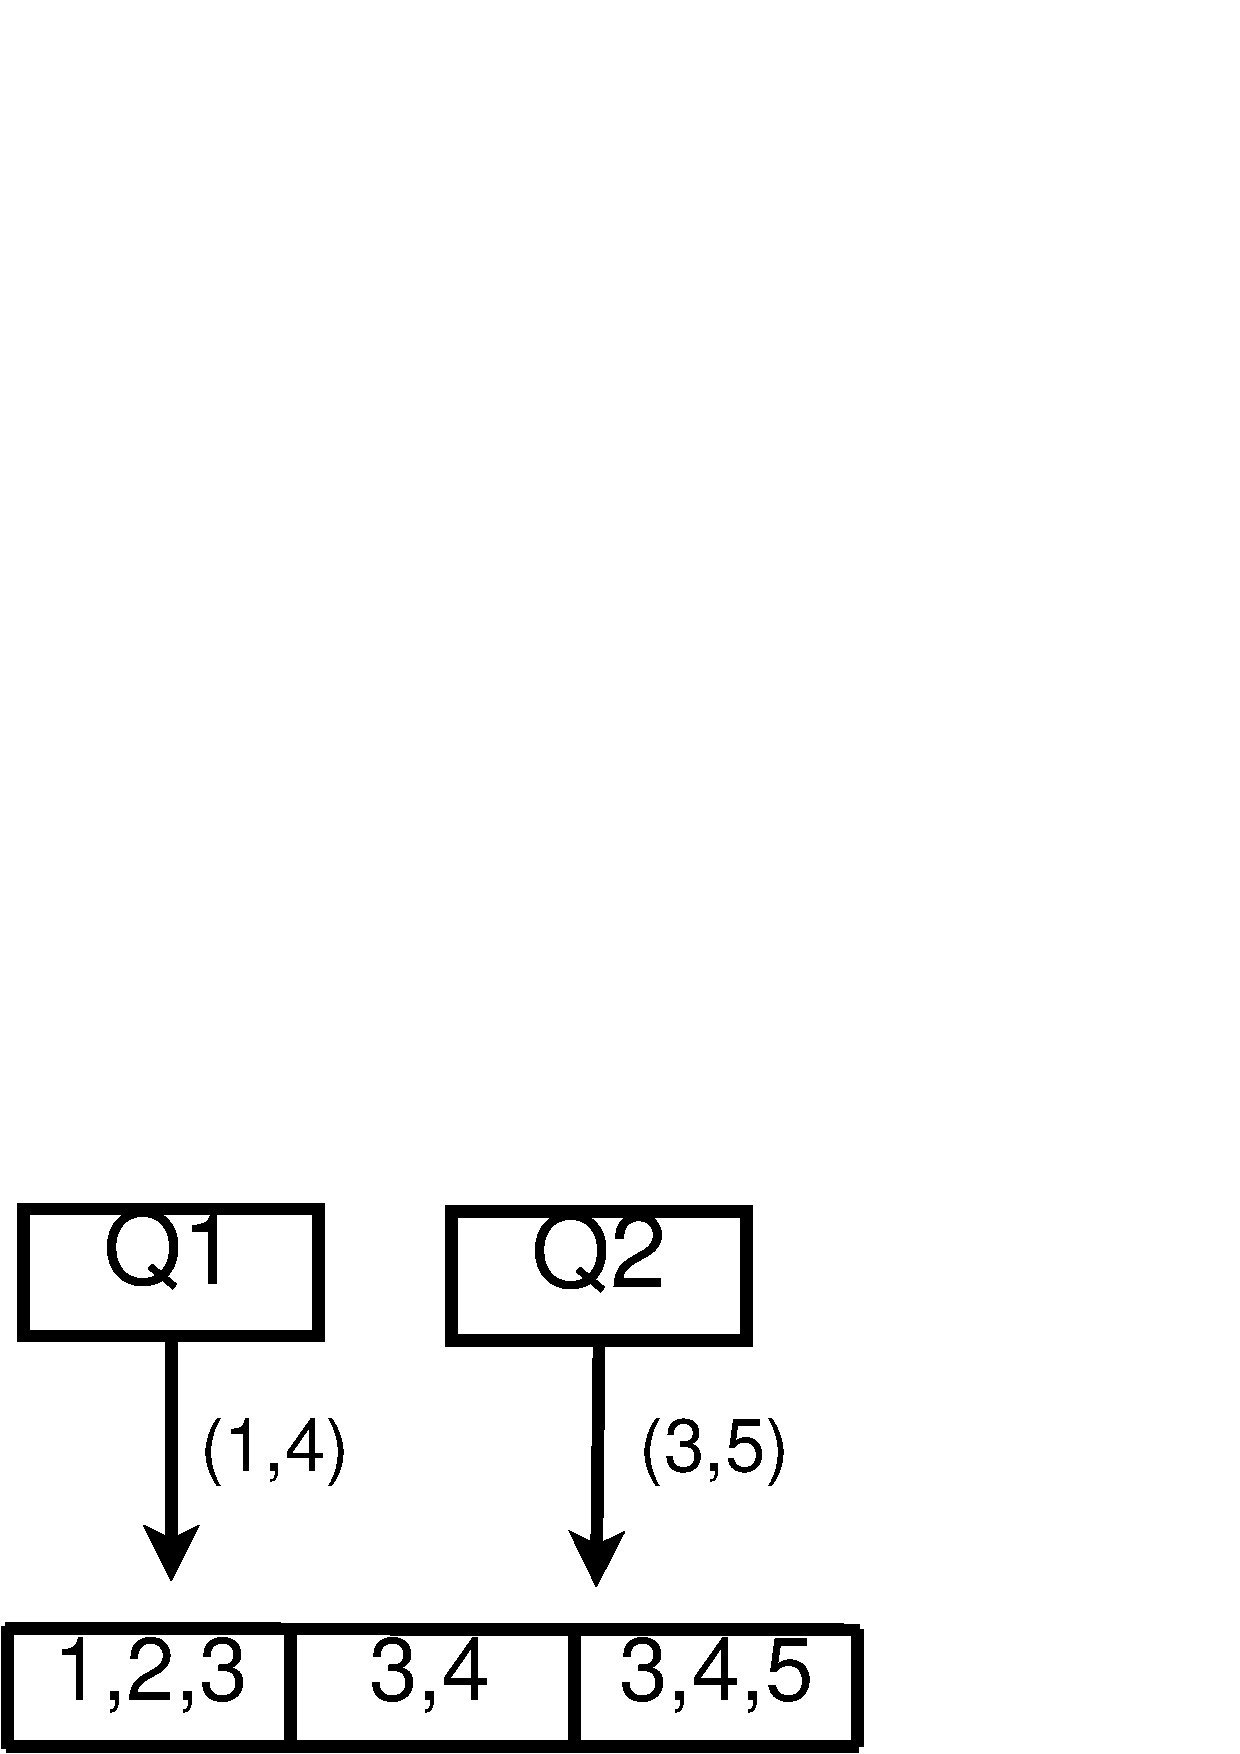
\includegraphics[width=0.25\textwidth]{figures/cacheQueries.pdf}
% % % % % % % % 	\caption{Queries}
% % % % % % % %   \label{fig:cacheQueries}
% % % % % % % % \end{figure}
% % % % % % % % 
% % % % % % % % 
% % % % % % % % \subsubsection{SP Results - facts}
% % % % % % % % \ffh{just to remember what facts I have available}
% % % % % % % % \begin{itemize}
% % % % % % % % \item number of times each node in query has been relevant to: 
% % % % % % % % \begin{itemize}
% % % % % % % % \item a cache hit
% % % % % % % % \item a query result
% % % % % % % % \end{itemize}
% % % % % % % % \item number of times source/target -nodes has been used in a query
% % % % % % % % \item sub-paths which are popular in query results (connected nodes which all "`score high"')
% % % % % % % % \end{itemize}
% % % % % % % % 
% % % % % % % % 
% % % % % % % % ---------------
% % % % % % % % 
% % % % % % % % \begin{deff}
% % % % % % % % A \textbf{SP Cache element} is a list $\left(v_s,v_{1},...,v_t\right)$ of vertices where $v_s/v_t$ are the start/end vertices of the list. $v_s$ is connected with $v_t$ by a shortest path defined by the vertices between $v_s$ and $v_t$ in the list.
% % % % % % % % \end{deff}
% % % % % % % % 
% % % % % % % % The cache is a set $\left\{SP_0,...,SP_n\right\}$ of SP cache elements. 
% % % % % % % % 
% % % % % % % % \begin{deff}
% % % % % % % % Cache replacement: Given two otherwise equal SP results, i.e. having the same length and having the same \textbf{value} (by some scoring mechanism defined for cache replacement) the SP result already in the cache will stay in the cache.
% % % % % % % % \end{deff}
% % % % % % % % 
% % % % % % % % 
% % % % % % % % \ffh{what other SSSP algorithms might be useful in comparing speed difference between cache and SP calculation?}
% % % % % % % % 
% % % % % % % % \ffh{Argue that since storing map data is cheap (little space required) but calculating SP is very expensive, then using the same, or more, space for cache than used for map data makes sense.}
% % % % % % % % 
% % % % % % % % ------------------
% % % % % % % % 
% % % % % % % % 
% % % % % % % % To initially identify basic weaknesses and strong points of our ideas we validate some of our simpler assumptions using a uniform random model(URM) together with a simple 'map',the graph in figure \ref{fig:simplemap}, enabling us to clearly reason about the advantages expected when using server side caching of \spath queries. By using the simple map (fig.\ref{fig:simplemap}) and a URM together with we can reason about the probabilities that a specific query will occur. Figure \ref{fig:queryprob} illustrates the number of queries possible for a map with 2,3, and 5 locations for figure \ref{fig:queryprob}A, \ref{fig:queryprob}B, and \ref{fig:queryprob}C respectively. Each line underneath each of the simple graphs represents two possible queries (A->B, B->A). The number of shortest-path queries possible on a tree-graph with n vertices is $n*(n-1)$. The probability of seeing any one query, $q_i$ is then $P(q_i | n) = (n*n-1)^{-1}$
% % % % % % % % 
% % % % % % % % \begin{figure}
% % % % % % % %   \center
% % % % % % % % 	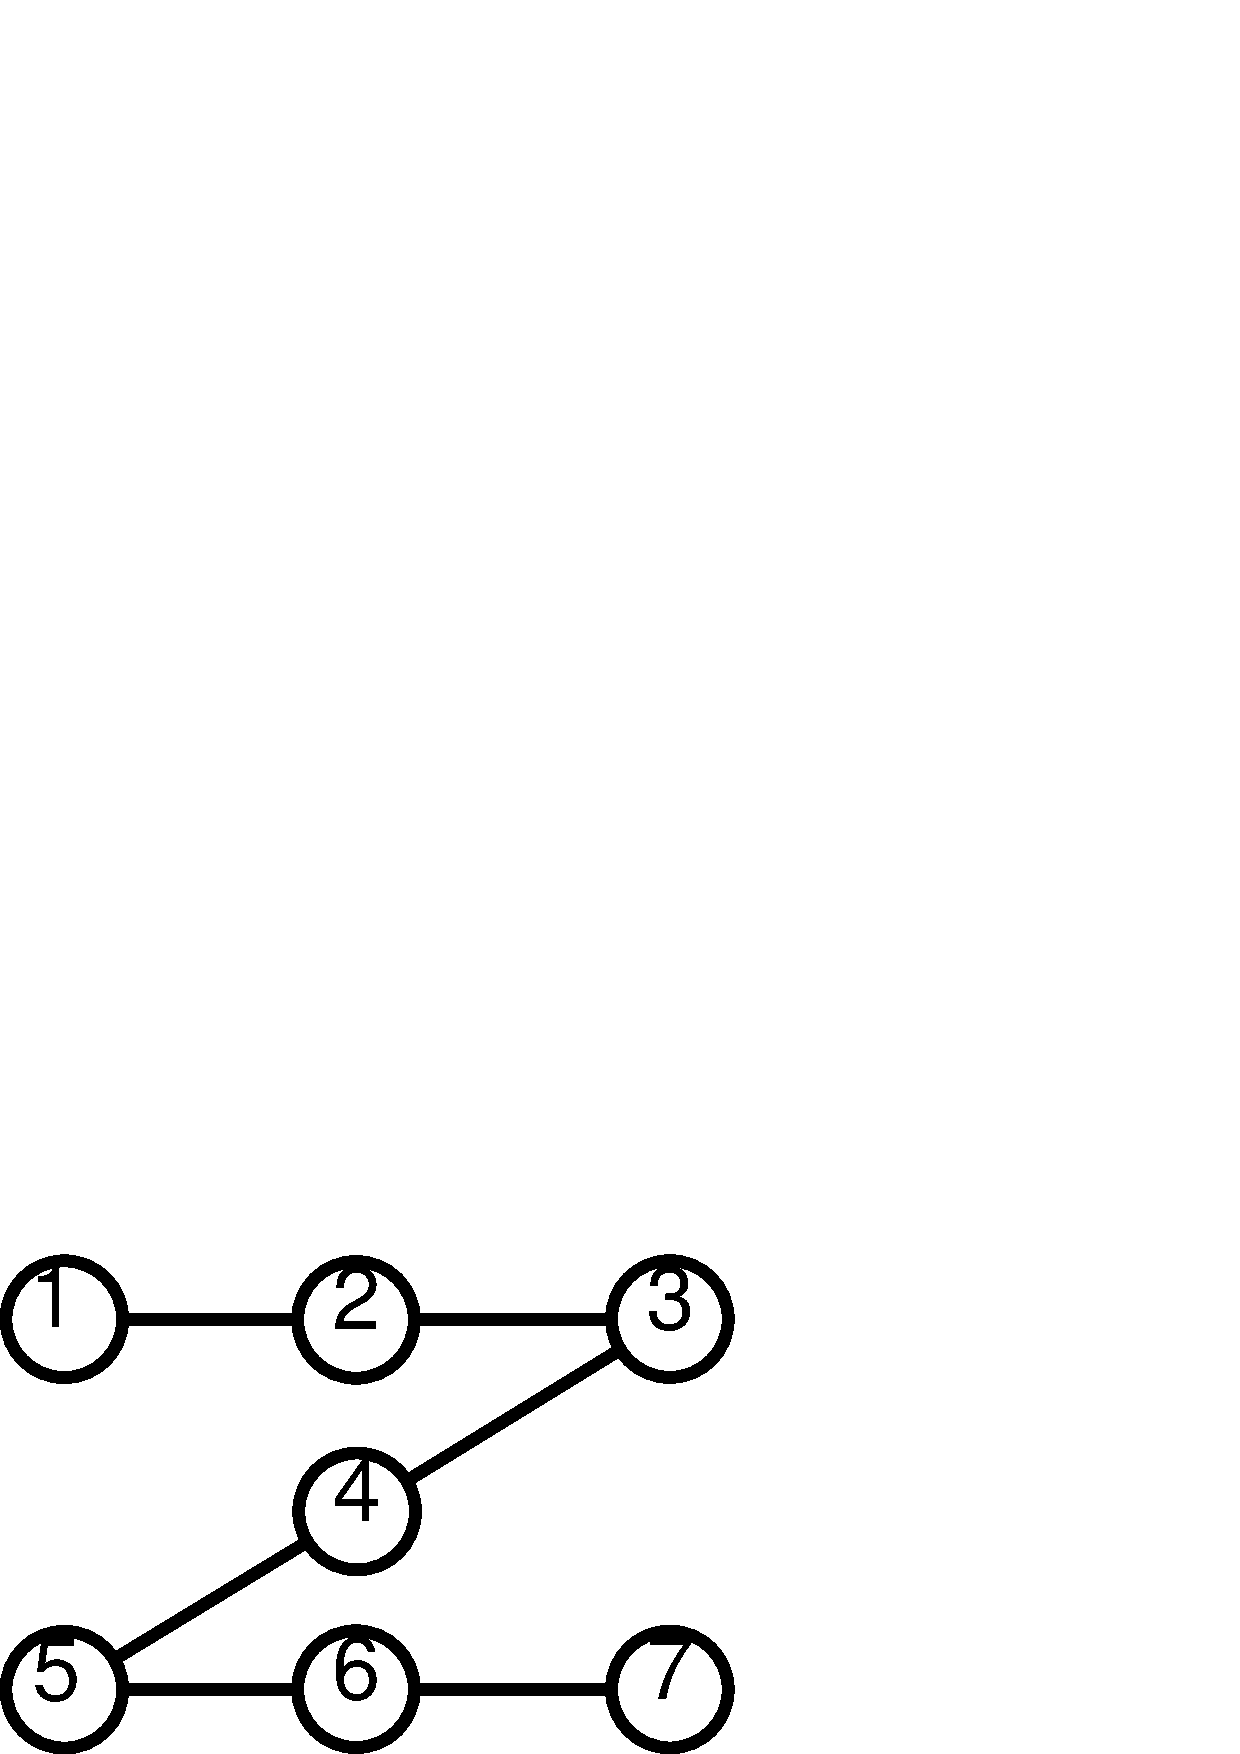
\includegraphics[width=0.25\textwidth]{figures/simpleMap.pdf}
% % % % % % % % 	\caption{Simple map}
% % % % % % % %   \label{fig:simplemap}
% % % % % % % % \end{figure}
% % % % % % % % 
% % % % % % % % \begin{figure}
% % % % % % % %   \center
% % % % % % % % 	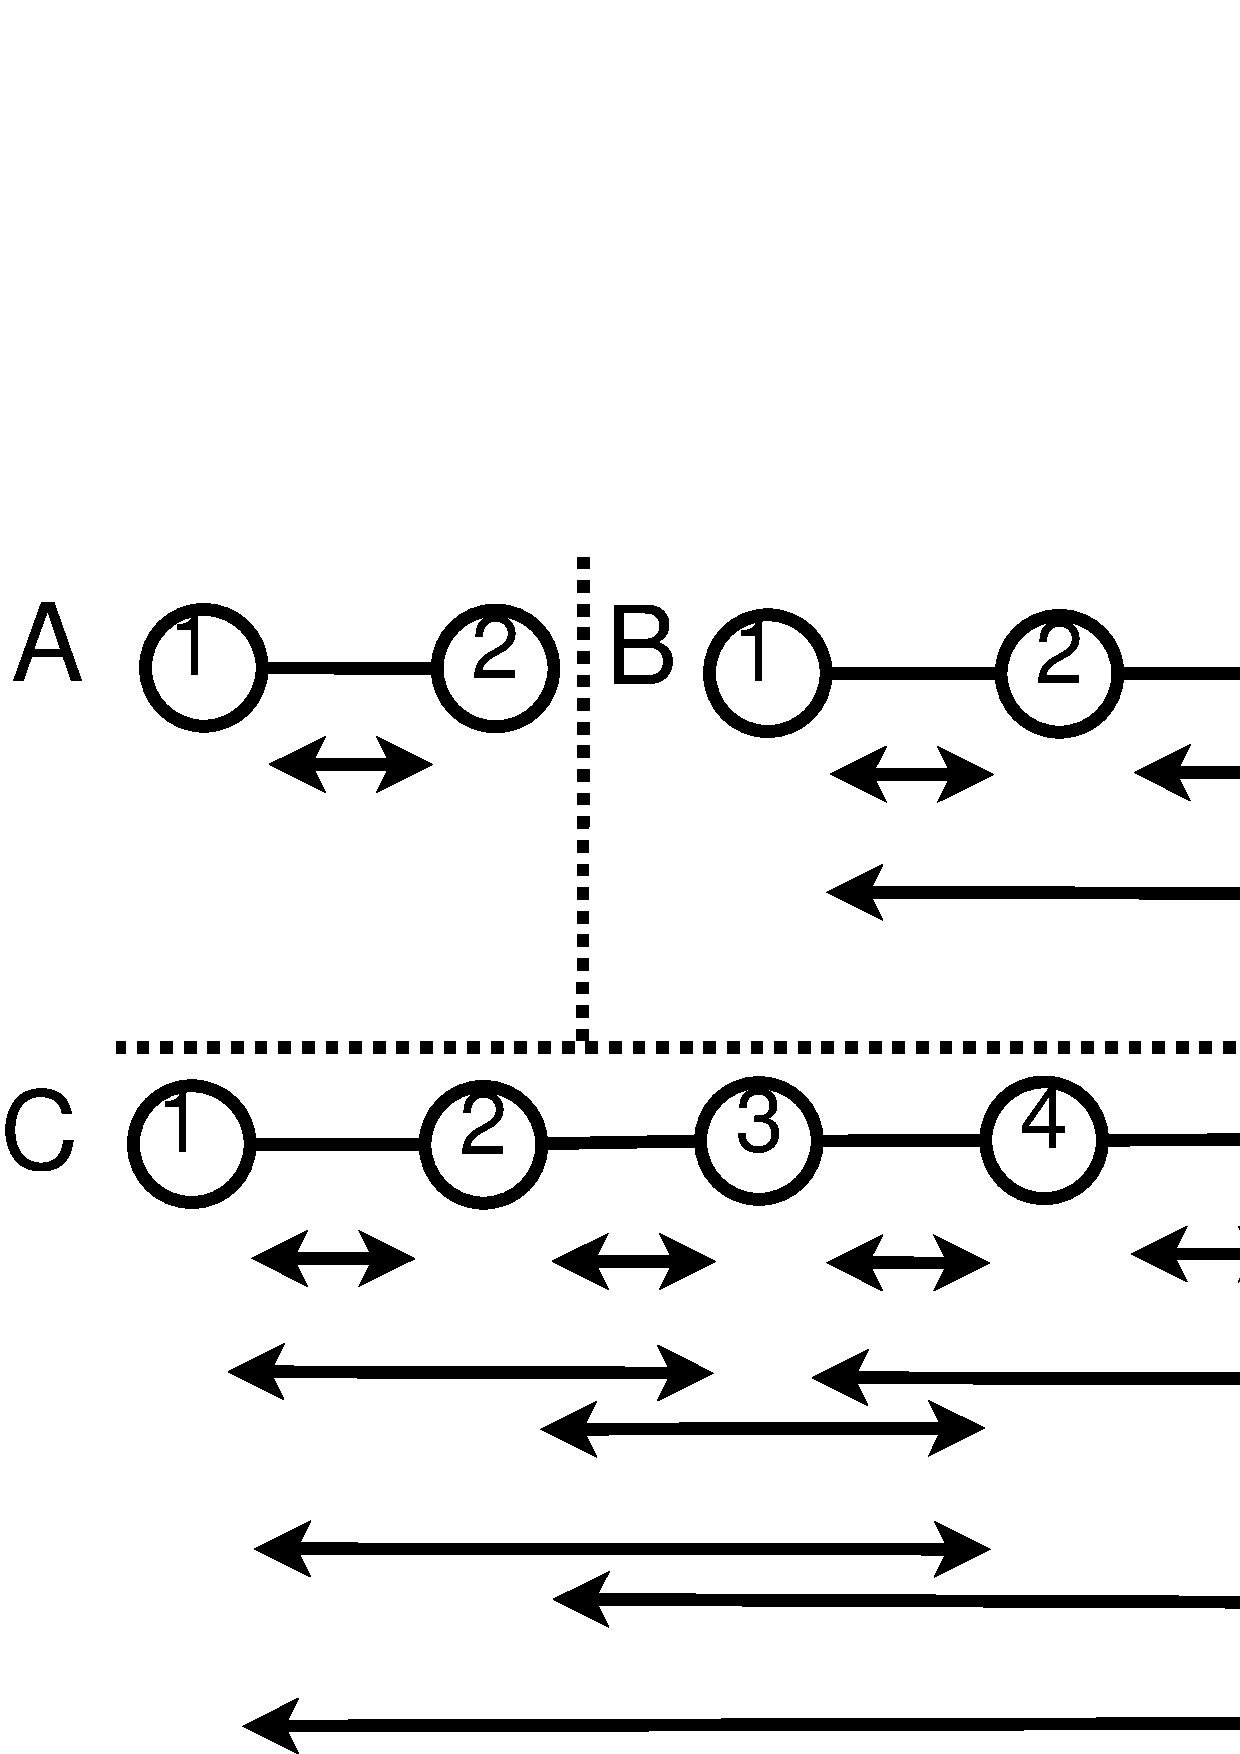
\includegraphics[width=0.25\textwidth]{figures/queryprob.pdf}
% % % % % % % % 	\caption{Number of queries possible}
% % % % % % % %   \label{fig:queryprob}
% % % % % % % % \end{figure}
% % % % % % % % 
